\section{Erweiterung auf Graphen im zweidimensionalen Raum}
\label{gcn_erweiterung}

Die Ansätze von~\citeauthor{Defferrard} aus Kapitel~\ref{spektraler_faltungsoperator} und von~\citeauthor{gcn} aus Kapitel~\ref{graph_convolutional_networks} zeigen konkurrenzfähige Resultate auf einer Reihe von Datensätzen auf Graphen (\vgl{}~\cite{Defferrard, gcn}).
So erreicht das \gls{GCN} \zB{} in der teilweise-überwachten Knotenklassifizierung von \emph{Referenzgraphen}, \dhe{} einer Menge von Knoten, die Dokumente über eine Reihe von Bag-of-Words-Merkmalen repräsentieren und (ungerichtet) über dessen Referenzierungen miteinander verbunden sind, beachtliche Ergebnisse und schneidet in diesen sogar knapp besser ab als über die Tschebyschow-Approximation mit $K=2$ und $K=3$~\cite{gcn}.

Die spektrale Faltung auf Graphen entspricht einer Generalisierung der Faltung klassischer \glspl{CNN} auf zweidimensionalen Bildern~\cite{gcn_review}.
Es ist jedoch anzumerken, dass die spektrale Faltung im Gegensatz zur klassischen Faltung auf einem regulären Gitter insbesondere rotationsinvariant ist.
Das ist in der Regel für generelle Graphen keine Schwäche, schließlich kann den Knoten \bzw{} Kanten eines Graphen, kodiert als Adjazenzmatrix, keine Örtlichkeit \bzw{} Richtung (wie links, rechts, oben oder unten) zugeordnet werden.
Die Rotationsinvarianz kann folglich sowohl als Einschränkung als auch als Vorteil interpretiert werden, abhängig von dem Problem, welches man betrachtet~\cite{Defferrard}.

\begin{figure}[t]
\centering
\subfigure[Reguläres Gitter]{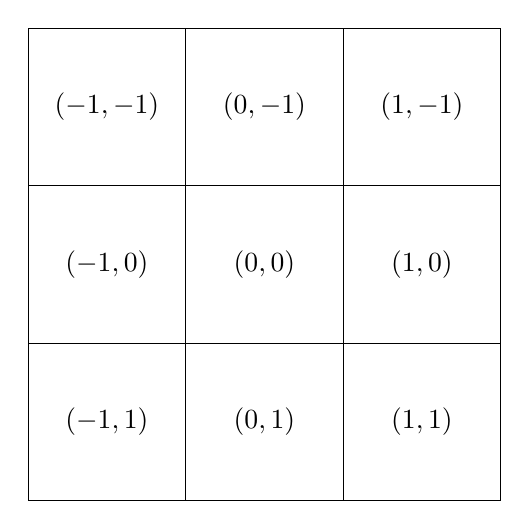
\begin{tikzpicture}
  \draw (-3, -3) rectangle (-1, -1) node[pos=0.5] {$\left(-1, 1\right)$};
  \draw (-1, -3) rectangle (1, -1)  node[pos=0.5] {$\left(0, 1\right)$};
  \draw (1, -3)  rectangle (3, -1)  node[pos=0.5] {$\left(1, 1\right)$};
  \draw (-3, -1) rectangle (-1, 1)  node[pos=0.5] {$\left(-1, 0\right)$};
  \draw (-1, -1) rectangle (1, 1)   node[pos=0.5] {$\left(0, 0\right)$};
  \draw (1, -1)  rectangle (3, 1)   node[pos=0.5] {$\left(1, 0\right)$};
  \draw (-3, 1)  rectangle (-1, 3)  node[pos=0.5] {$\left(-1, -1\right)$};
  \draw (-1, 1)  rectangle (1, 3)   node[pos=0.5] {$\left(0, -1\right)$};
  \draw (1, 1)   rectangle (3, 3)   node[pos=0.5] {$\left(1, -1\right)$};
\end{tikzpicture}
}
\hspace{1cm}
\subfigure[Graphrepräsentation]{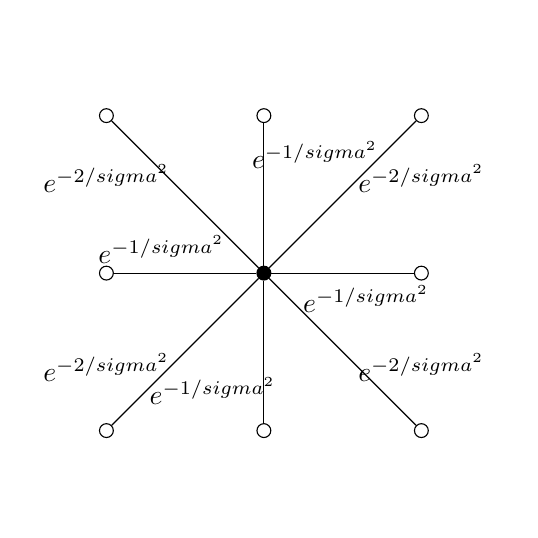
\begin{tikzpicture}
  \tikzstyle{node}=[circle,draw, minimum width=5pt, inner sep=0pt, fill=white]
  \tikzstyle{root}=[fill=black]
  \fill [white] (-3, -3) rectangle (3, 3) node {};  % Zentriere vertikal.

  \node[node] (00) at (-2, 2) {};
  \node[node] (01) at (0, 2) {};
  \node[node] (02) at (2, 2) {};
  \node[node] (10) at (-2, 0) {};
  \node[node, root] (11) at (0,0) {};
  \node[node] (12) at (2, 0) {};
  \node[node] (20) at (-2, -2) {};
  \node[node] (21) at (0, -2) {};
  \node[node] (22) at (2, -2) {};

  \path (10) edge node[shift={(-0.3, 0.3)}]  {$e^{-1/\gls{sigma}^2}$} (11);
  \path (11) edge node[shift={(0.3, -0.33)}]  {$e^{-1/\gls{sigma}^2}$} (12);
  \path (01) edge node[shift={(0.65, 0.5)}]   {$e^{-1/\gls{sigma}^2}$} (11);
  \path (11) edge node[shift={(-0.65, -0.5)}] {$e^{-1/\gls{sigma}^2}$} (21);
  \path (00) edge node[shift={(-1, 0.2)}]    {$e^{-2/\gls{sigma}^2}$} (11);
  \path (02) edge node[shift={(1, 0.2)}]     {$e^{-2/\gls{sigma}^2}$} (11);
  \path (11) edge node[shift={(1, -0.2)}]    {$e^{-2/\gls{sigma}^2}$} (22);
  \path (20) edge node[shift={(-1, -0.2)}]   {$e^{-2/\gls{sigma}^2}$} (11);
\end{tikzpicture}
}
  \caption[Graphrepräsentation eines regulären Gitters]{Illustration (a) eines $3 \times 3$ großen regulären Gitters zentriert um den Punkt $\left(0, 0\right)$ und (b) dessen lokale Nachbarschaft der entsprechenden Graphrepräsentation mit einer Konnektivität von $8$ bei horizontalen \bzw{} vertikalen Kantengewichten $\exp\left(-1/\gls{sigma}^2\right) \in \gls{R}$ und respektive $\exp\left(-2/\gls{sigma}^2\right) \in \gls{R}$ bei den Diagonalen.}
\label{fig:gcn_review}
\end{figure}


Im Kontext dieser Arbeit, dem Lernen auf Graphen im zweidimensionalen euklidschen Raum, bei denen Graphknoten eine eindeutige Position besitzen, ist die Rotationsinvarianz weitestgehend unerwünscht.
Das kann leicht verifiziert werden, indem wir den Filter des \glspl{GCN} auf einer Graphrepräsentation eines Gitters mit Abstand $\left\|1\right\|_2$ visualisieren (vgl. Abbildung~\ref{fig:gcn_review}).
Diese Repräsentation entspricht damit genau dem Problem der zweidimensionalen Faltung auf Bildern mit einer Filtergröße von $3 \times 3$.
Hier zeigt sich jedoch besonders deutlich die Limitierung des Netzes durch die Rotationsinvarianz.
Wohingegen wir bei klassischen \glspl{CNN} $3 \times 3$ unterschiedliche Parameter mit eindeutiger Örtlichkeit auf den benachbarten Bildpixeln trainieren, reduziert sich der Filter des \glspl{GCN} (vereinfacht ohne Normalisierung mit $\gls{Dtilde}^{-1/2}$) effektiv zu einer Filtermatrix der Form
\begin{equation*}
  \begin{bmatrix}
    ce^{-2/\gls{sigma}^2} & ce^{-1/\gls{sigma}^2} & ce^{-2/\gls{sigma}^2}\\
    ce^{-1/\gls{sigma}^2} & c & ce^{-1/\gls{sigma}^2}\\
    ce^{-2/\gls{sigma}^2} & ce^{-1/\gls{sigma}^2} & ce^{-2/\gls{sigma}^2}
  \end{bmatrix} = c \begin{bmatrix}
    e^{-2/\gls{sigma}^2} & e^{-1/\gls{sigma}^2} & e^{-2/\gls{sigma}^2}\\
    e^{-1/\gls{sigma}^2} & 1 & e^{-1/\gls{sigma}^2}\\
    e^{-2/\gls{sigma}^2} & e^{-1/\gls{sigma}^2} & e^{-2/\gls{sigma}^2}
  \end{bmatrix}
\end{equation*}
mit einem einzigen trainierbaren Parameter $c \in \gls{R}$ bei horizontalen \bzw{} vertikalen Kantengewichten $\exp\left(-1/\gls{sigma}^2\right) \in \gls{R}$ \bzw{} $\exp\left(-2/\gls{sigma}^2\right) \in \gls{R}$ bei den Diagonalen.
Damit reduziert sich das Training einer Faltungsschicht eines solchen \glspl{GCN} letztendlich auf eine Skalarmultiplikation.
Es scheint schwer vorstellbar mit diesem Ansatz komplexe Probleme wie \zB{} das Segmentieren eines Bildes zu lösen~(\vgl{}~\cite{gcn_review}).
Ein Vergleich zwischen der spektralen Faltung auf regulären Gittergraphen und der klassischen zweidimensionalen Faltung auf Bildern wird der spektralen Faltung aber nicht gerecht, schließlich wurden die klassischen \glspl{CNN} speziell für die Anwendung auf Gittern entwickelt.
So ist es zu erwarten, dass durch die Formulierung einer Faltung für generelle Graphen gewisse Einschränkungen in Kauf genommen werden müssen.
Im Folgenden lässt sich der Faltungsoperator der \glspl{GCN} aber insofern modifizieren, dass sich dieser für beliebige Graphen in einem zweidimensionalen euklischen Raum äquivalent zu der klassischen Formulierung auf regulären Gittern verhält.

\subsection{Partitionierung}
\label{partitionierung}

\section{Partitionierung}

\section{Partitionierung}

\section{Partitionierung}

\input{figures/partitionierung}

\subsection{Grundlagen}

\begin{itemize}
  \item ungerichtete Distanzadjazenzmatrix $\gls{Adist} \in \gls{R+}^{N \times N} = {\left(a\right)}_{ij}$
  \item (lokal) normalisierte ungerichtete Distanzadjazenzmatrix $\gls{Adistnorm} \in \gls{R+}^{N \times N} = {\left(\tilde a\right)}_{ij}$
  \item gerichtete Winkeladjazenzmatrix $\gls{Arad} \in \gls{R+}^{N \times N} = {\left(\alpha\right)}_{ij}$
  \item Input-Featurematrix $\gls{F} \in \gls{R}^{N \times X} = {\left(f\right)}_{ij}$
  \item Output-Featurematrix $\gls{Fout} \in \gls{R}^{N \times Y} = {\left(f^{\prime}\right)}_{ij}$
  \item Anzahl Partitionen $P \in \gls{N}$
  \item Gewichtstensor $\ma{W} \in \gls{R}^{\left(P + 1\right) \times X \times Y} = {\left(w\right)}_{ijw}$
\end{itemize}

\subsection{Faltung}

\begin{equation}
  f^{\prime}_{iy} = \sum_{x = 1}^X \tilde a_{ii} \cdot f_{ix} \cdot w_{\left(P +1\right)xy} \sum_{n = 1, n \neq i}^N \tilde a_{in} \cdot f_{nx} \cdot b^K_P\left(\alpha_{in}, x, y\right)
\end{equation}
wobei $b_P^K$ eine B-Spline-Kurve.

Es ist anzumerken, dass im Summanden der betrachtete Knoten übersprungen wird, da für diesen ein Wert in der Winkelmatrix keinen Sinn ergibt.
Er wird daher in der Faltung jeweils einzeln mit einem Gewicht multipliziert und dazuaddiert.

\subsection{B-Spline-Kurven}

$b_P^K \colon \left]0, 2\pi\right] \times \left\{1, \ldots, X \right\} \times \left\{1, \ldots, Y\right\} \to \gls{R}$ ist eine B-Spline-Kurve der Ordnung $K \in \gls{N}$ auf den Kantenwinkeln des Graphen.
Bemerke, dass wir $0$ für Winkel aussschließen und stattdessen den Winkel $2\pi$ benutzen, so dass wir nicht mit der Bedeutung von $0$ bei Adjazenzmatrizen in die Quere kommen.
\begin{equation}
  b_P^K\left(\alpha, x, y \right) = \sum_{p=1}^P w_{pxy} \cdot e_p^K\left(\alpha\right)
\end{equation}
wobei die Basisfunktion $e_p^K$ rekursiv über $K$ definiert ist mit Initialisierung
\begin{equation}
  e_p^1\left(\alpha\right) = \begin{cases}
    1, & \text{wenn }\alpha \in \left] t\left(p-1\right), t\left(p\right)\right]\text{,}\\
    0, & \text{sonst}
  \end{cases}
\end{equation}
und Rekursionsschritt
\begin{equation}
  e_p^k\left(\alpha\right) = \frac{\alpha - t\left(p - 1\right)}{t\left(p+k-2\right) - t\left(p - 1\right)} e_p^{k-1}\left(\alpha\right) + \frac{t\left(i\left(p + k - 1\right)\right) - \alpha}{t\left(p+k - 1\right) - t\left(p\right)} e_{i\left(p+1\right)}^{k-1}\left(\alpha\right)
\end{equation}
wobei $t \colon \gls{N} \to \gls{R}$ mit $t\left(p\right) = 2\pi\frac{p}{P}$ und $i\left(p\right) = \gls{modulo}\left(p-1, P\right) + 1$.
Es ist anzumerken, dass wir $t$ und $i$ dabei für den Rekursionsschritt über die Grenze $P$ hinaus definieren.
Das hilft uns, die B-Spline-Kurve \emph{kreisförmig} abzuschließen.

Je größer $K$ gesetzt wird, umso mehr Anteile anderer benachbarter Stützpunkte fließen in die Berechnung mit ein.
Die Größe von $K$ wird deshalb auch oft \emph{lokale Kontrollierbarkeit} genannt.

\subsubsection{Beispiel mit $P=4$}

\input{figures/bspline-basis}

\subsubsection{Effiziente Berechnung für $K=2$}

Wir können für $K=2$ die Basis-Berechnung durch
\begin{equation}
  e_p^2\left(\alpha\right) = \begin{cases}
    \min\left(\frac{P}{2\pi} \alpha - p + 1, 0\right), & \text{wenn }\alpha \leq t\left(p\right)\text{,}\\
    \min\left(-\frac{P}{2\pi} \alpha + p + 1, 0\right), & \text{sonst}
  \end{cases}
\end{equation}
vereinfachen.

\begin{proof}
  Aufsteigende Gerade der Dreiecksfunktion für $p$, $1 \leq p \leq P$, ist definiert durch
  \begin{equation}
    \frac{\alpha - t\left(p-1\right)}{t\left(p\right) - t\left(p-1\right)} = \frac{P\left(\alpha - t\left(p-1\right)\right)}{2\pi} = \frac{P\alpha - 2\pi\left(p-1\right)}{2\pi} = \frac{P}{2\pi}\alpha - p + 1.
  \end{equation}
  $\min \left(\frac{P}{2\pi} \alpha - p + 1, 0\right)$ beschreibt damit die linke Seite des Dreiecks.
  Analog für absteigende Gerade.
\end{proof}

Die Fallunterscheidung ist unnötig, wir können uns einfach immer für das Minimum der beiden entscheiden.
Die Grafik zeigt dies ziemlich eindeutig.
Das ergibt letztendlich
\begin{equation}
  e_p^2\left(\alpha\right) = \min \left( \min\left(\frac{P}{2\pi} \alpha - p + 1, 0\right), \min\left(-\frac{P}{2\pi} \alpha + p + 1, 0\right) \right)\text{.}
\end{equation}

\input{figures/bspline-basis-k-2}

Wir haben bisher noch nicht den \emph{Kreis} geschlossen mit unserer Formel.

Das können wir aber leicht tun, indem wir unsere absteigenden Geraden um $2\pi$ nach links verschieben und daraus wiederum das Minimum von $0$ ziehen.
Dann sind diese Geraden außer für $p = P$ im Gültigkeitsbereich der Funktion allesamt $0$.
Wir können demnach aus unserer bisherigen Formel und der verschobenen Gerade das Maximum ziehen.
Wir erhalten
\begin{equation}
\begin{split}
  e_p^2\left(\alpha\right) = \max \biggr( & \min \left( \min\left(\frac{P}{2\pi} \alpha - p + 1, 0\right), \min\left(-\frac{P}{2\pi} \alpha + p + 1, 0\right) \right),\\
  & \min \left(-\frac{P}{2\pi} \left( \alpha + 2\pi \right) + p + 1, 0\right) \biggr)\text{.}
\end{split}
\end{equation}

\subsection{Tensorimplementierung}

\begin{equation}
\begin{split}
  \gls{Fout} = & \ {\left(\gls{Adistnorm}\right)}_{ii} \cdot \gls{F} \cdot \ma{W}_{P+1}\\
  & + \sum_{p=1}^P \gls{Adistnorm} \gls{hadamard} e^K_p\left(\gls{Arad}\right) \cdot \gls{F} \cdot \ma{W}_{p}
\end{split}
\end{equation}

\gls{Adistnorm} enthält einmal nur die Diagonale und einmal alles ohne Diagonale.

\newpage


\subsection{Grundlagen}

\begin{itemize}
  \item ungerichtete Distanzadjazenzmatrix $\gls{Adist} \in \gls{R+}^{N \times N} = {\left(a\right)}_{ij}$
  \item (lokal) normalisierte ungerichtete Distanzadjazenzmatrix $\gls{Adistnorm} \in \gls{R+}^{N \times N} = {\left(\tilde a\right)}_{ij}$
  \item gerichtete Winkeladjazenzmatrix $\gls{Arad} \in \gls{R+}^{N \times N} = {\left(\alpha\right)}_{ij}$
  \item Input-Featurematrix $\gls{F} \in \gls{R}^{N \times X} = {\left(f\right)}_{ij}$
  \item Output-Featurematrix $\gls{Fout} \in \gls{R}^{N \times Y} = {\left(f^{\prime}\right)}_{ij}$
  \item Anzahl Partitionen $P \in \gls{N}$
  \item Gewichtstensor $\ma{W} \in \gls{R}^{\left(P + 1\right) \times X \times Y} = {\left(w\right)}_{ijw}$
\end{itemize}

\subsection{Faltung}

\begin{equation}
  f^{\prime}_{iy} = \sum_{x = 1}^X \tilde a_{ii} \cdot f_{ix} \cdot w_{\left(P +1\right)xy} \sum_{n = 1, n \neq i}^N \tilde a_{in} \cdot f_{nx} \cdot b^K_P\left(\alpha_{in}, x, y\right)
\end{equation}
wobei $b_P^K$ eine B-Spline-Kurve.

Es ist anzumerken, dass im Summanden der betrachtete Knoten übersprungen wird, da für diesen ein Wert in der Winkelmatrix keinen Sinn ergibt.
Er wird daher in der Faltung jeweils einzeln mit einem Gewicht multipliziert und dazuaddiert.

\subsection{B-Spline-Kurven}

$b_P^K \colon \left]0, 2\pi\right] \times \left\{1, \ldots, X \right\} \times \left\{1, \ldots, Y\right\} \to \gls{R}$ ist eine B-Spline-Kurve der Ordnung $K \in \gls{N}$ auf den Kantenwinkeln des Graphen.
Bemerke, dass wir $0$ für Winkel aussschließen und stattdessen den Winkel $2\pi$ benutzen, so dass wir nicht mit der Bedeutung von $0$ bei Adjazenzmatrizen in die Quere kommen.
\begin{equation}
  b_P^K\left(\alpha, x, y \right) = \sum_{p=1}^P w_{pxy} \cdot e_p^K\left(\alpha\right)
\end{equation}
wobei die Basisfunktion $e_p^K$ rekursiv über $K$ definiert ist mit Initialisierung
\begin{equation}
  e_p^1\left(\alpha\right) = \begin{cases}
    1, & \text{wenn }\alpha \in \left] t\left(p-1\right), t\left(p\right)\right]\text{,}\\
    0, & \text{sonst}
  \end{cases}
\end{equation}
und Rekursionsschritt
\begin{equation}
  e_p^k\left(\alpha\right) = \frac{\alpha - t\left(p - 1\right)}{t\left(p+k-2\right) - t\left(p - 1\right)} e_p^{k-1}\left(\alpha\right) + \frac{t\left(i\left(p + k - 1\right)\right) - \alpha}{t\left(p+k - 1\right) - t\left(p\right)} e_{i\left(p+1\right)}^{k-1}\left(\alpha\right)
\end{equation}
wobei $t \colon \gls{N} \to \gls{R}$ mit $t\left(p\right) = 2\pi\frac{p}{P}$ und $i\left(p\right) = \gls{modulo}\left(p-1, P\right) + 1$.
Es ist anzumerken, dass wir $t$ und $i$ dabei für den Rekursionsschritt über die Grenze $P$ hinaus definieren.
Das hilft uns, die B-Spline-Kurve \emph{kreisförmig} abzuschließen.

Je größer $K$ gesetzt wird, umso mehr Anteile anderer benachbarter Stützpunkte fließen in die Berechnung mit ein.
Die Größe von $K$ wird deshalb auch oft \emph{lokale Kontrollierbarkeit} genannt.

\subsubsection{Beispiel mit $P=4$}

\begin{center}
\begin{tikzpicture}
  \begin{axis}[xmax=4.5,
               xmin=0,
               ymin=0,
               ymax=1.25,
               xlabel={$\alpha$},
               ylabel={$e_p^1$},
               xtick={1, 2, 3, 4},
               xticklabels={$\frac{\pi}{2}$, $\pi$, $\frac{3\pi}{2}$, $2\pi$},
               ytick={1},
               axis equal,
               axis x line=center,
               axis y line=center,
               xlabel style={below right},
               ylabel style={above left},
               legend pos=outer north east]
    \addplot [ultra thick, brown] coordinates {(0,1)(1,1)};
    \addlegendentry{$p = 1$}
    \addplot [ultra thick, blue] coordinates {(1,1)(2,1)};
    \addlegendentry{$p = 2$}
    \addplot [ultra thick, red] coordinates {(2,1)(3,1)};
    \addlegendentry{$p = 3$}
    \addplot [ultra thick, green] coordinates {(3,1)(4,1)};
    \addlegendentry{$p = 4$}
  \end{axis}
\end{tikzpicture}
\end{center}

\begin{center}
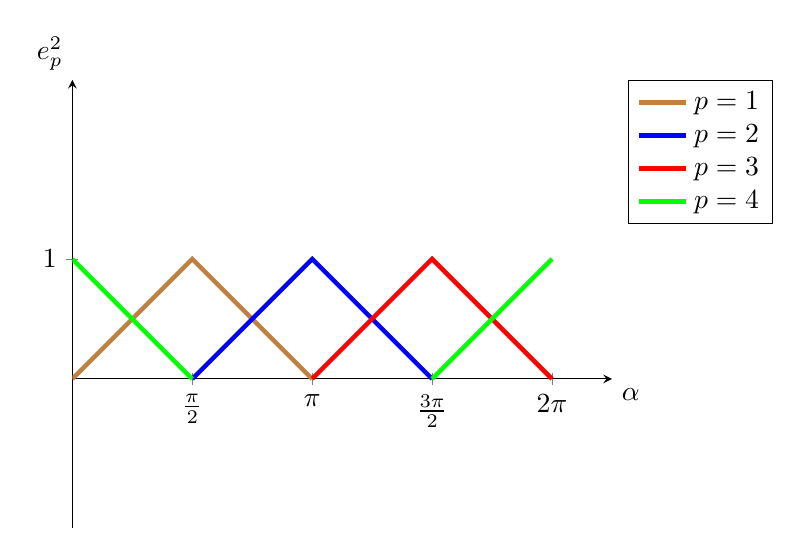
\begin{tikzpicture}
  \begin{axis}[xmax=4.5,
               xmin=0,
               ymin=0,
               ymax=1.25,
               xlabel={$\alpha$},
               ylabel={$e_p^2$},
               xtick={1, 2, 3, 4},
               xticklabels={$\frac{\pi}{2}$, $\pi$, $\frac{3\pi}{2}$, $2\pi$},
               ytick={1},
               axis equal,
               axis x line=center,
               axis y line=center,
               xlabel style={below right},
               ylabel style={above left},
               legend pos=outer north east]
    \addplot [ultra thick, brown] coordinates {(0,0)(1,1)(2,0)};
    \addlegendentry{$p = 1$}
    \addplot [ultra thick, blue] coordinates {(1,0)(2,1)(3,0)};
    \addlegendentry{$p = 2$}
    \addplot [ultra thick, red] coordinates {(2,0)(3,1)(4,0)};
    \addlegendentry{$p = 3$}
    \addplot [ultra thick, green] coordinates {(3,0)(4,1)};
    \addlegendentry{$p = 4$}
    \addplot [ultra thick, green] coordinates {(0,1)(1,0)};
  \end{axis}
\end{tikzpicture}
\end{center}


\subsubsection{Effiziente Berechnung für $K=2$}

Wir können für $K=2$ die Basis-Berechnung durch
\begin{equation}
  e_p^2\left(\alpha\right) = \begin{cases}
    \min\left(\frac{P}{2\pi} \alpha - p + 1, 0\right), & \text{wenn }\alpha \leq t\left(p\right)\text{,}\\
    \min\left(-\frac{P}{2\pi} \alpha + p + 1, 0\right), & \text{sonst}
  \end{cases}
\end{equation}
vereinfachen.

\begin{proof}
  Aufsteigende Gerade der Dreiecksfunktion für $p$, $1 \leq p \leq P$, ist definiert durch
  \begin{equation}
    \frac{\alpha - t\left(p-1\right)}{t\left(p\right) - t\left(p-1\right)} = \frac{P\left(\alpha - t\left(p-1\right)\right)}{2\pi} = \frac{P\alpha - 2\pi\left(p-1\right)}{2\pi} = \frac{P}{2\pi}\alpha - p + 1.
  \end{equation}
  $\min \left(\frac{P}{2\pi} \alpha - p + 1, 0\right)$ beschreibt damit die linke Seite des Dreiecks.
  Analog für absteigende Gerade.
\end{proof}

Die Fallunterscheidung ist unnötig, wir können uns einfach immer für das Minimum der beiden entscheiden.
Die Grafik zeigt dies ziemlich eindeutig.
Das ergibt letztendlich
\begin{equation}
  e_p^2\left(\alpha\right) = \min \left( \min\left(\frac{P}{2\pi} \alpha - p + 1, 0\right), \min\left(-\frac{P}{2\pi} \alpha + p + 1, 0\right) \right)\text{.}
\end{equation}

\begin{figure}
  \centering
  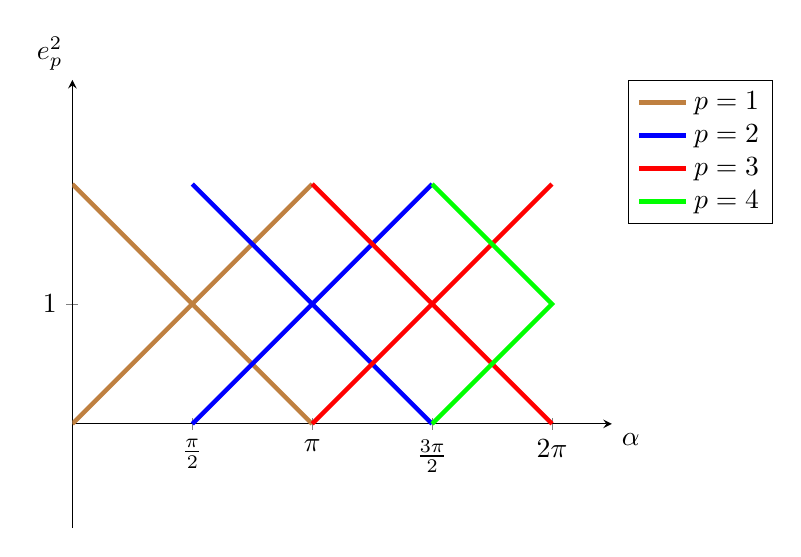
\begin{tikzpicture}
    \begin{axis}[xmax=4.5,
                 xmin=0,
                 ymin=0,
                 ymax=2,
                 xlabel={$\alpha$},
                 ylabel={$e_p^2$},
                 xtick={1, 2, 3, 4},
                 xticklabels={$\frac{\pi}{2}$, $\pi$, $\frac{3\pi}{2}$, $2\pi$},
                 ytick={1},
                 axis equal,
                 axis x line=center,
                 axis y line=center,
                 xlabel style={below right},
                 ylabel style={above left},
                 legend pos=outer north east]
      \addplot [ultra thick, brown] coordinates {(0,0)(2,2)(1,1)(0,2)(2,0)};
      \addlegendentry{$p = 1$}
      \addplot [ultra thick, blue] coordinates {(1,0)(3,2)(2,1)(1,2)(3,0)};
      \addlegendentry{$p = 2$}
      \addplot [ultra thick, red] coordinates {(2,0)(4,2)(3,1)(2,2)(4,0)};
      \addlegendentry{$p = 3$}
      \addplot [ultra thick, green] coordinates {(3,0)(4,1)(3,2)};
      \addlegendentry{$p = 4$}
    \end{axis}
  \end{tikzpicture}
\end{figure}


Wir haben bisher noch nicht den \emph{Kreis} geschlossen mit unserer Formel.

Das können wir aber leicht tun, indem wir unsere absteigenden Geraden um $2\pi$ nach links verschieben und daraus wiederum das Minimum von $0$ ziehen.
Dann sind diese Geraden außer für $p = P$ im Gültigkeitsbereich der Funktion allesamt $0$.
Wir können demnach aus unserer bisherigen Formel und der verschobenen Gerade das Maximum ziehen.
Wir erhalten
\begin{equation}
\begin{split}
  e_p^2\left(\alpha\right) = \max \biggr( & \min \left( \min\left(\frac{P}{2\pi} \alpha - p + 1, 0\right), \min\left(-\frac{P}{2\pi} \alpha + p + 1, 0\right) \right),\\
  & \min \left(-\frac{P}{2\pi} \left( \alpha + 2\pi \right) + p + 1, 0\right) \biggr)\text{.}
\end{split}
\end{equation}

\subsection{Tensorimplementierung}

\begin{equation}
\begin{split}
  \gls{Fout} = & \ {\left(\gls{Adistnorm}\right)}_{ii} \cdot \gls{F} \cdot \ma{W}_{P+1}\\
  & + \sum_{p=1}^P \gls{Adistnorm} \gls{hadamard} e^K_p\left(\gls{Arad}\right) \cdot \gls{F} \cdot \ma{W}_{p}
\end{split}
\end{equation}

\gls{Adistnorm} enthält einmal nur die Diagonale und einmal alles ohne Diagonale.

\newpage


\subsection{Grundlagen}

\begin{itemize}
  \item ungerichtete Distanzadjazenzmatrix $\gls{Adist} \in \gls{R+}^{N \times N} = {\left(a\right)}_{ij}$
  \item (lokal) normalisierte ungerichtete Distanzadjazenzmatrix $\gls{Adistnorm} \in \gls{R+}^{N \times N} = {\left(\tilde a\right)}_{ij}$
  \item gerichtete Winkeladjazenzmatrix $\gls{Arad} \in \gls{R+}^{N \times N} = {\left(\alpha\right)}_{ij}$
  \item Input-Featurematrix $\gls{F} \in \gls{R}^{N \times X} = {\left(f\right)}_{ij}$
  \item Output-Featurematrix $\gls{Fout} \in \gls{R}^{N \times Y} = {\left(f^{\prime}\right)}_{ij}$
  \item Anzahl Partitionen $P \in \gls{N}$
  \item Gewichtstensor $\ma{W} \in \gls{R}^{\left(P + 1\right) \times X \times Y} = {\left(w\right)}_{ijw}$
\end{itemize}

\subsection{Faltung}

\begin{equation}
  f^{\prime}_{iy} = \sum_{x = 1}^X \tilde a_{ii} \cdot f_{ix} \cdot w_{\left(P +1\right)xy} \sum_{n = 1, n \neq i}^N \tilde a_{in} \cdot f_{nx} \cdot b^K_P\left(\alpha_{in}, x, y\right)
\end{equation}
wobei $b_P^K$ eine B-Spline-Kurve.

Es ist anzumerken, dass im Summanden der betrachtete Knoten übersprungen wird, da für diesen ein Wert in der Winkelmatrix keinen Sinn ergibt.
Er wird daher in der Faltung jeweils einzeln mit einem Gewicht multipliziert und dazuaddiert.

\subsection{B-Spline-Kurven}

$b_P^K \colon \left]0, 2\pi\right] \times \left\{1, \ldots, X \right\} \times \left\{1, \ldots, Y\right\} \to \gls{R}$ ist eine B-Spline-Kurve der Ordnung $K \in \gls{N}$ auf den Kantenwinkeln des Graphen.
Bemerke, dass wir $0$ für Winkel aussschließen und stattdessen den Winkel $2\pi$ benutzen, so dass wir nicht mit der Bedeutung von $0$ bei Adjazenzmatrizen in die Quere kommen.
\begin{equation}
  b_P^K\left(\alpha, x, y \right) = \sum_{p=1}^P w_{pxy} \cdot e_p^K\left(\alpha\right)
\end{equation}
wobei die Basisfunktion $e_p^K$ rekursiv über $K$ definiert ist mit Initialisierung
\begin{equation}
  e_p^1\left(\alpha\right) = \begin{cases}
    1, & \text{wenn }\alpha \in \left] t\left(p-1\right), t\left(p\right)\right]\text{,}\\
    0, & \text{sonst}
  \end{cases}
\end{equation}
und Rekursionsschritt
\begin{equation}
  e_p^k\left(\alpha\right) = \frac{\alpha - t\left(p - 1\right)}{t\left(p+k-2\right) - t\left(p - 1\right)} e_p^{k-1}\left(\alpha\right) + \frac{t\left(i\left(p + k - 1\right)\right) - \alpha}{t\left(p+k - 1\right) - t\left(p\right)} e_{i\left(p+1\right)}^{k-1}\left(\alpha\right)
\end{equation}
wobei $t \colon \gls{N} \to \gls{R}$ mit $t\left(p\right) = 2\pi\frac{p}{P}$ und $i\left(p\right) = \gls{modulo}\left(p-1, P\right) + 1$.
Es ist anzumerken, dass wir $t$ und $i$ dabei für den Rekursionsschritt über die Grenze $P$ hinaus definieren.
Das hilft uns, die B-Spline-Kurve \emph{kreisförmig} abzuschließen.

Je größer $K$ gesetzt wird, umso mehr Anteile anderer benachbarter Stützpunkte fließen in die Berechnung mit ein.
Die Größe von $K$ wird deshalb auch oft \emph{lokale Kontrollierbarkeit} genannt.

\subsubsection{Beispiel mit $P=4$}

\begin{center}
\begin{tikzpicture}
  \begin{axis}[xmax=4.5,
               xmin=0,
               ymin=0,
               ymax=1.25,
               xlabel={$\alpha$},
               ylabel={$e_p^1$},
               xtick={1, 2, 3, 4},
               xticklabels={$\frac{\pi}{2}$, $\pi$, $\frac{3\pi}{2}$, $2\pi$},
               ytick={1},
               axis equal,
               axis x line=center,
               axis y line=center,
               xlabel style={below right},
               ylabel style={above left},
               legend pos=outer north east]
    \addplot [ultra thick, brown] coordinates {(0,1)(1,1)};
    \addlegendentry{$p = 1$}
    \addplot [ultra thick, blue] coordinates {(1,1)(2,1)};
    \addlegendentry{$p = 2$}
    \addplot [ultra thick, red] coordinates {(2,1)(3,1)};
    \addlegendentry{$p = 3$}
    \addplot [ultra thick, green] coordinates {(3,1)(4,1)};
    \addlegendentry{$p = 4$}
  \end{axis}
\end{tikzpicture}
\end{center}

\begin{center}
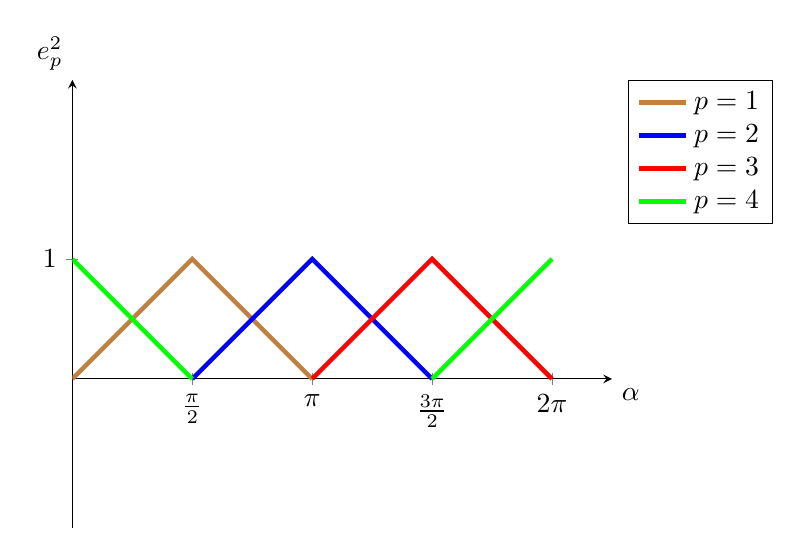
\begin{tikzpicture}
  \begin{axis}[xmax=4.5,
               xmin=0,
               ymin=0,
               ymax=1.25,
               xlabel={$\alpha$},
               ylabel={$e_p^2$},
               xtick={1, 2, 3, 4},
               xticklabels={$\frac{\pi}{2}$, $\pi$, $\frac{3\pi}{2}$, $2\pi$},
               ytick={1},
               axis equal,
               axis x line=center,
               axis y line=center,
               xlabel style={below right},
               ylabel style={above left},
               legend pos=outer north east]
    \addplot [ultra thick, brown] coordinates {(0,0)(1,1)(2,0)};
    \addlegendentry{$p = 1$}
    \addplot [ultra thick, blue] coordinates {(1,0)(2,1)(3,0)};
    \addlegendentry{$p = 2$}
    \addplot [ultra thick, red] coordinates {(2,0)(3,1)(4,0)};
    \addlegendentry{$p = 3$}
    \addplot [ultra thick, green] coordinates {(3,0)(4,1)};
    \addlegendentry{$p = 4$}
    \addplot [ultra thick, green] coordinates {(0,1)(1,0)};
  \end{axis}
\end{tikzpicture}
\end{center}


\subsubsection{Effiziente Berechnung für $K=2$}

Wir können für $K=2$ die Basis-Berechnung durch
\begin{equation}
  e_p^2\left(\alpha\right) = \begin{cases}
    \min\left(\frac{P}{2\pi} \alpha - p + 1, 0\right), & \text{wenn }\alpha \leq t\left(p\right)\text{,}\\
    \min\left(-\frac{P}{2\pi} \alpha + p + 1, 0\right), & \text{sonst}
  \end{cases}
\end{equation}
vereinfachen.

\begin{proof}
  Aufsteigende Gerade der Dreiecksfunktion für $p$, $1 \leq p \leq P$, ist definiert durch
  \begin{equation}
    \frac{\alpha - t\left(p-1\right)}{t\left(p\right) - t\left(p-1\right)} = \frac{P\left(\alpha - t\left(p-1\right)\right)}{2\pi} = \frac{P\alpha - 2\pi\left(p-1\right)}{2\pi} = \frac{P}{2\pi}\alpha - p + 1.
  \end{equation}
  $\min \left(\frac{P}{2\pi} \alpha - p + 1, 0\right)$ beschreibt damit die linke Seite des Dreiecks.
  Analog für absteigende Gerade.
\end{proof}

Die Fallunterscheidung ist unnötig, wir können uns einfach immer für das Minimum der beiden entscheiden.
Die Grafik zeigt dies ziemlich eindeutig.
Das ergibt letztendlich
\begin{equation}
  e_p^2\left(\alpha\right) = \min \left( \min\left(\frac{P}{2\pi} \alpha - p + 1, 0\right), \min\left(-\frac{P}{2\pi} \alpha + p + 1, 0\right) \right)\text{.}
\end{equation}

\begin{figure}
  \centering
  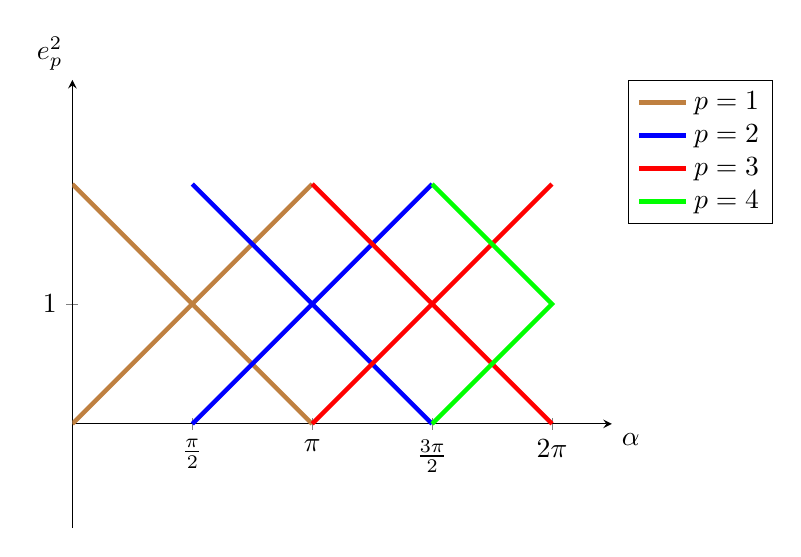
\begin{tikzpicture}
    \begin{axis}[xmax=4.5,
                 xmin=0,
                 ymin=0,
                 ymax=2,
                 xlabel={$\alpha$},
                 ylabel={$e_p^2$},
                 xtick={1, 2, 3, 4},
                 xticklabels={$\frac{\pi}{2}$, $\pi$, $\frac{3\pi}{2}$, $2\pi$},
                 ytick={1},
                 axis equal,
                 axis x line=center,
                 axis y line=center,
                 xlabel style={below right},
                 ylabel style={above left},
                 legend pos=outer north east]
      \addplot [ultra thick, brown] coordinates {(0,0)(2,2)(1,1)(0,2)(2,0)};
      \addlegendentry{$p = 1$}
      \addplot [ultra thick, blue] coordinates {(1,0)(3,2)(2,1)(1,2)(3,0)};
      \addlegendentry{$p = 2$}
      \addplot [ultra thick, red] coordinates {(2,0)(4,2)(3,1)(2,2)(4,0)};
      \addlegendentry{$p = 3$}
      \addplot [ultra thick, green] coordinates {(3,0)(4,1)(3,2)};
      \addlegendentry{$p = 4$}
    \end{axis}
  \end{tikzpicture}
\end{figure}


Wir haben bisher noch nicht den \emph{Kreis} geschlossen mit unserer Formel.

Das können wir aber leicht tun, indem wir unsere absteigenden Geraden um $2\pi$ nach links verschieben und daraus wiederum das Minimum von $0$ ziehen.
Dann sind diese Geraden außer für $p = P$ im Gültigkeitsbereich der Funktion allesamt $0$.
Wir können demnach aus unserer bisherigen Formel und der verschobenen Gerade das Maximum ziehen.
Wir erhalten
\begin{equation}
\begin{split}
  e_p^2\left(\alpha\right) = \max \biggr( & \min \left( \min\left(\frac{P}{2\pi} \alpha - p + 1, 0\right), \min\left(-\frac{P}{2\pi} \alpha + p + 1, 0\right) \right),\\
  & \min \left(-\frac{P}{2\pi} \left( \alpha + 2\pi \right) + p + 1, 0\right) \biggr)\text{.}
\end{split}
\end{equation}

\subsection{Tensorimplementierung}

\begin{equation}
\begin{split}
  \gls{Fout} = & \ {\left(\gls{Adistnorm}\right)}_{ii} \cdot \gls{F} \cdot \ma{W}_{P+1}\\
  & + \sum_{p=1}^P \gls{Adistnorm} \gls{hadamard} e^K_p\left(\gls{Arad}\right) \cdot \gls{F} \cdot \ma{W}_{p}
\end{split}
\end{equation}

\gls{Adistnorm} enthält einmal nur die Diagonale und einmal alles ohne Diagonale.

\newpage


Sei \gls{G} ein Graph im zweidimensionalen euklidschen Raum, eindeutig definiert über dessen Adjazenzmatrizen $\gls{Adist} \in {\left[0, 1\right)}^{N \times N}$ und $\gls{Arad} \in {\left[0, 2\pi\right]}^{N \times N}$.
Dann lässt sich \gls{G} in $P \in \gls{N}$ Bereiche ${\left\{\gls{A}_p\right\}}_{p=0}^{P-1}$ \emph{partitionieren}, sodass
\begin{equation*}
  {\left(\gls{A}_p\right)}_{ij} \coloneqq \begin{cases}
    {\left(\gls{Adist}\right)}_{ij}, & \text{wenn } {\left(\gls{Arad}\right)}_{ij} \in \left(2\pi p/P, 2\pi\left(p+1\right)/P\right]\\
    0, & \text{sonst.}
  \end{cases}
\end{equation*}
Damit beschreiben die Matrizen ${\left\{\gls{A}_p\right\}}_{p=0}^{P-1}$ disjunkte Partitionen der Kanten des Graphen \gls{G} abhängig von ihren Ausrichtungen im Raum mit $\gls{Adist} = \sum_{p=0}^{P-1} \gls{A}_p$.
$\gls{A}_p$ ist insbesondere nicht symmetrisch, da ${\left(\gls{Arad}\right)}_{ij} \neq {\left(\gls{Arad}\right)}_{ji}$ für alle $\gls{v}_i, \gls{v}_j \in \gls{V}$ mit $\gls{v}_j \in \gls{Neighbor}\left(\gls{v}_i\right)$.
Abbildung~\ref{fig:partitionierung} veranschaulicht den Prozess der Partitionierung.
Mit $P = 8$ erhalten die jeweiligen Bereiche \zB{} einen gleichmäßigen Innenwinkel der Größe $\pi/4$.

\paragraph{Faltungsoperator}
\label{partitionierung_faltungsoperator}

Es lässt sich analog zu Kapitel~\ref{graph_convolutional_networks} ein Faltungsoperator definieren, bei dem nun jeder Partition ein eigener frei trainierbarer Parameter zugeordnet wird.
Der Parameter einer Partition hat damit folglich eine eindeutige Örtlichkeitszuweisung über das Intervall \bzw{} den Bereich der Richtungen seiner Kanten.
Analog zu~\eqref{eq:gcn_renorm} muss dafür zuerst die (Re-)normalisierung der Form
\begin{equation*}
  \gls{Ddisttilde}^{-\frac{1}{2}}\gls{Adisttilde}\gls{Ddisttilde}^{-\frac{1}{2}} = \gls{Ddisttilde}^{-1} + \sum_{p=0}^{P-1} \gls{Ddisttilde}^{-\frac{1}{2}}\gls{A}_p\gls{Ddisttilde}^{-\frac{1}{2}}
\end{equation*}
mit $\gls{Adisttilde} \coloneqq \gls{Adist} + \gls{I}$ und ${\left(\gls{Ddisttilde}\right)}_{ii} \coloneqq \sum_{j=1}^N {\left(\gls{Adisttilde}\right)}_{ij}$ durchgeführt werden.
Dies lässt sich mit Hilfe von $\gls{Adist} = \sum_{p=0}^{P-1} \gls{A}_p$ und $\gls{Ddisttilde}^{-1/2}\gls{Ddisttilde}^{-1/2} = \gls{Ddisttilde}^{-1}$ verifizieren.
Im Folgenden sei $\gls{Atilde}_p \coloneqq \gls{Ddisttilde}^{-1/2}\gls{A}_p\gls{Ddisttilde}^{-1/2}$ für $p \in \left\{0, \ldots, P-1 \right\}$ und $\gls{Atilde}_P \coloneqq \gls{Ddisttilde}^{-1}$.
Dann folgt für den Faltungsoperatur $\ve{f}_{\mathrm{in}} \star \ve{\hat g}$ auf Graphen im zweidimensionalen euklidschen Raum, dass dieser über
\begin{equation}
  \ve{f}_{\mathrm{in}} \star \ve{\hat g} \approx \sum_{p=0}^P c_p \gls{Atilde}_p \ve{f}_{\mathrm{in}}
  \label{eq:partitionierung_faltung}
\end{equation}
mit den freien Parametern ${\left[c_0, \ldots, c_P\right]}^{\top} \in \gls{R}^{P+1}$ beschrieben werden kann.
\\\\
Es stellt sich heraus, dass die Faltung in~\eqref{eq:partitionierung_faltung} auf den Partitionen eines regulären Gittergraphen mit $P=8$ äquivalent zu der klassischen Faltung auf einem regulären Gitter mit Filtergröße $3 \times 3$ ist.
Sei dafür \gls{G} ein (unendlicher) regulärer Gittergraph bei einer Konnektivität von $8$ und $\ve{f}_{\mathrm{in}}$ Merkmalsvektor auf dem Graphen mit Koordinatenindexnotation ${\left(\ve{f}_{\mathrm{in}}\right)}_{x,y}$.
  Die klassische Faltung \gls{conv2d} an einem Gitterpunkt $\left(x, y\right)$ ist damit gegeben als
\begin{equation*}
  {\gls{conv2d}\left({\ve{f}_{\mathrm{in}}}\right)}_{x,y} = \sum_{i,j \in \left\{1, 2, 3\right\}} {\left(\ve{f}_{\mathrm{in}}\right)}_{x+i-2, y+j-2} \gls{W}_{i, j},
\end{equation*}
wobei $\gls{W} \in \gls{R}^{3 \times 3}$ eine Filtermatrix der Größe $3 \times 3$ ist.
Da \gls{Adisttilde} ein reguläres Gitter beschreibt sind die Einträge ihrer Matrixreihen äquivalent unter unterschiedlicher Permutation und folglich sind die Einträge auf der Diagonalen von \gls{Ddisttilde} identisch (\oBdA{} entfällt hier die Randknotenbetrachtung).
Aufgrund der Partitionierung von \gls{Adist} in $8$ disjunkte Bereiche ${\left\{\gls{Atilde}_p\right\}}_{p=0}^7$ enthält $\gls{Atilde}_p$ genau einen Eintrag pro Matrixreihe korrespondierend zu einer Kante des regulären Gitters.
Für $p \in \left\{1, 3, 5, 7\right\}$ beschreibt $\gls{Atilde}_p$ die horizontalen und vertikalen Kanten des Graphen mit jeweils gleichen Einträgen $\theta_0 \in \gls{R}$.
Analog verweist $\gls{Atilde}_p$ für $p \in \left\{0, 2, 4, 6\right\}$ auf die diagonalen Kanten des Graphen mit den festen Einträgen $\theta_1 \in \gls{R}$.
Sei weiterhin \oBdA{} $\theta_2 \coloneqq {\left(\gls{Ddisttilde}^{-1}\right)}_{ii}$ für beliebiges $i \in \left\{0, \ldots, N\right\}$.
Mit der Zuordnung
\begin{equation*}
  \gls{W} = \begin{bmatrix}
    c_6\theta_1 & c_7\theta_0 & c_0\theta_1\\
    c_5\theta_0 & c_8\theta_2 & c_1\theta_0\\
    c_4\theta_1 & c_3\theta_0 & c_2\theta_1
  \end{bmatrix}
\end{equation*}
  für den Faltungsoperator $\ve{f}_{\mathrm{in}} \star \ve{\hat g}$ aus~\eqref{eq:partitionierung_faltung} mit den Parametern ${\left[c_0, \ldots, c_8\right]}^{\top} \in \gls{R}^9$
folgt damit sofort die Äquivalenz zu $\gls{conv2d}\left(\ve{f}_{\mathrm{in}}\right)$ auf regulären Gittern.

\paragraph{Implementierung}
\label{partitionierung_implementierung}

Analog zu~\eqref{eq:gcn_tensor} lässt sich die Faltung für Merkmalsmatrizen $\ma{F}_{\mathrm{in}} \in \gls{R}^{N \times M_{\mathrm{in}}}$ und $\ma{F}_{\mathrm{out}} \in \gls{R}^{N \times M_{\mathrm{out}}}$ über einem Filtertensor $\gls{W} \in \gls{R}^{\left(P+1\right) \times M_{\mathrm{in}} \times M_{\mathrm{out}}}$ als
\begin{equation*}
  \ma{F}_{\mathrm{out}} \coloneqq \sum_{p=0}^P \gls{Atilde}_p\ma{F}_{\mathrm{in}}\gls{W}_{p+1}
\end{equation*}
beschreiben.
Es ist anzumerken, dass die Multiplikation mit den dünnbesetzten partitionierten Adjazenzmatrizen ${\left\{\gls{Atilde}_p\right\}}_{p=0}^P$ extrem effizient ist, da $\left|\gls{E}_p\right| \ll \left|\gls{E}\right|$ und insbesondere $\sum_{p=0}^P \left|\gls{E}_p\right| = \left|\gls{E}\right| + N$ gilt, wobei $\gls{E}_p \in \gls{V} \times \gls{V}$ die Kantenmenge der Adjazenzmatrix $\gls{Atilde}_p$ beschreibt.
Die Laufzeit erhöht sich jedoch im Vergleich zu~\eqref{eq:gcn_tensor} durch die $P$-fache Multiplikation mit der Filtermatrix $\gls{W}_p$ zu $\gls{O}\left(PM_{\mathrm{in}}M_{\mathrm{out}}\left|\gls{E}\right|\right)$.
\\\\
Obwohl die Faltung auf den Partitionen eines Graphen insbesondere durch die Äquivalenz zur klassischen Faltung auf regulären Gittern vielversprechend erscheint, gehen dabei dennoch Informationen über die Ausrichtung der Kanten im Raum verloren.
Kanten mit verschiedenen Richtungen im Intervall $\left(2\pi p/P, 2\pi \left(p+1\right)/P\right]$ landen jeweils in der gleichen Partition $p$, auch wenn sich diese \evtl{} extrem unterscheiden.
Eine Lösung zu diesem Problem ist sicherlich, $P$ insoweit zu erhöhen, dass die Innenwinkel der einzelnen Partitionen entsprechend klein werden.
Dies erscheint jedoch für beliebige, unbekannte Graphstrukturen nicht zwangsläufig sinnvoll.
Neben dem erhöhten Aufwand der Faltung erhalten wir im schlimmsten Fall viele Partitionsmatrizen $\gls{A}_p$, die eine Nullmatrix \ma{0} darstellen oder nur extrem wenige Kanten beinhalten.
Kleinste Veränderungen in den Ausrichtungen der Kanten sorgen dann schließlich dafür, dass eine komplett andere Filtermatrix angesprochen wird.
Ein dazu alternativ entwickelter Ansatz ist die Approximation des Filters über stückweise stetiger Polynome zwischen den Partitionsgrenzen des Graphen mit Hilfe von B-Spline-Kurven.

\subsection{Polynomielle Approximation über B-Spline-Kurven}
\label{bspline}

Eine \emph{offene B-Spline-Kurve} $\gls{spline}\left(t\right)$ beschreibt die stückweise polynomielle Approximation einer Kurve vom Grad $K$ über $m + 1$ Kontrollpunkten $\ve{d}_0, \ldots, \ve{d}_m \in \gls{R}^d$ auf dem Intervall $t \in \left[t_0, t_{m+1}\right)$ mit
\begin{equation}
  \gls{spline}\left(t\right) \coloneqq \sum_{i = 0}^m \ve{d}_i \gls{basis}_i^K\left(t\right),
    \label{eq:bspline}
\end{equation}
wobei ${\left\{\gls{basis}_i^K\right\}}_{i=0}^m$ die \emph{Basisfunktionen} zu einem \emph{Knotenvektor} $\ve{\tau} \in \gls{R}^{m+K+2}$ mit $\ve{\tau} \coloneqq {\left[t_0, \ldots, t_{m+K+1}\right]}^{\top}$, $t_i \leq t_{i+1}$~\cite{deBoor}.
Eine Basisfunktion $\gls{basis}_i^K \colon \left[t_0, t_{m+1}\right] \to \left[0, 1\right]$ ist dabei rekursiv über $K$ definiert mit der Initialisierung ($k=0$)
\begin{equation}
  \gls{basis}_i^0\left(t\right) \coloneqq \begin{cases}
    1, & \text{falls }t \in \left[t_i, t_{i+1}\right),\\
    0, & \text{sonst}
    \label{eq:bspline_basis_init}
  \end{cases}
\end{equation}
und dem Rekursionsschritt ($k - 1 \rightarrow k$)
\begin{equation}
  \gls{basis}_i^k\left(t\right) \coloneqq \frac{t-t_i}{t_{i+k} - t_i}\gls{basis}^{k-1}_i\left(t\right) + \frac{t_{i+k+1} - t}{t_{i+k+1} - t_{i+1}} \gls{basis}_{i+1}^{k-1}\left(t\right)
    \label{eq:bspline_basis_schritt}
\end{equation}
für $i \in \left\{ 0, \ldots, m \right\}$ und $k \in \left\{1, \ldots, K \right\}$~\cite{deBoor}.
Ein Kontrollpunkt $\ve{d}_i$ beeinflusst die Kurve damit lediglich im Intervall $t_i \leq t < t_{i+k}$.
Die Größe von $K$ wird deshalb auch oft \emph{lokale Kontrollierbarkeit} genannt.
Weiterhin gilt für die Aufsummierung der Basisfunktionen für $t \in \gls{R}$ und $k \in \gls{N}$, dass $\sum_{i=0}^m \gls{basis}_i^K\left(t\right) = 1$~\cite{deBoor}.

Wir können die Definition der B-Spline-Kurve $\gls{spline}\left(t\right)$ aus~\eqref{eq:bspline} nutzen, um sie aufbauend auf Kapitel~\ref{partitionierung} auf das Anwendungsgebiet eines stückweisen polynomiellen Filters $\gls{spline}\left(\alpha\right)$ auf die Richtungen \bzw{} Winkel eines Graphen \gls{G}, beschrieben durch \gls{Adist} und \gls{Arad}, zu übertragen.
Sei dafür $\gls{spline} \colon \left[0, 2\pi\right] \to \gls{R}$ eine B-Spline-Kurve auf den Winkeln der Graphkanten mit
\begin{equation}
  \gls{spline}\left(\alpha\right) \coloneqq \sum_{p=0}^{P-1} c_p N_p^K\left(\alpha\right),
\end{equation}
wobei die freien Parameter ${\left[c_0, \ldots, c_{P-1}\right]}^{\top} \in \gls{R}^{P}$ aus~\eqref{eq:partitionierung_faltung} nun die Koeffizienten der Basisfunktionen ${\left\{N_p^K\right\}}_{p=0}^{P-1}$ bilden.
Insbesondere definieren wir $\gls{spline}\left(0\right) \coloneqq 0$, da der Winkel $0$ in der Adjazenzmatrix $\gls{Arad}$ weiterhin angeben soll, dass $\left(\gls{v}_i, \gls{v}_j\right) \notin \gls{E}$.
Wir können uns $\gls{spline}\left(\alpha\right)$ damit weiterhin als eine $P$-fache Partitionierung von \gls{G} auf Basis seiner Kantenausrichtungen vorstellen, mit dem Unterschied, dass $\gls{spline}\left(\alpha\right)$ nun eine lokale Kontrollierbarkeit inne hält.
Kanten, die vorher zwar in einer gleichen Partition lagen, sich jedoch \evtl{} stark in ihrer Ausrichtung unterschieden, sind nun \enquote{eindeutig} differenzierbar über ihre abweichenden Auswertungen von ${\left\{\gls{basis}_p^K\right\}}_{p=0}^{P-1}$ \bzw{} ihrer Anteile von ${\left[c_0, \ldots, c_{P-1}\right]}^{\top}$ an $\gls{spline}\left(\alpha\right)$ entsprechend ihrer unterschiedlichen Winkel.

\begin{figure}[t]
\centering
\subfigure[$K=1$]{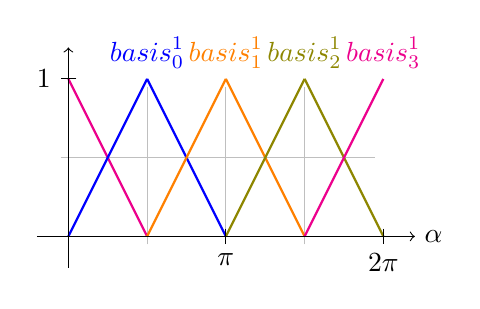
\begin{tikzpicture}
  \draw[color=lightgray] (-0.1, -0.1) grid (3.9, 1.9);

  \draw[thick,color=magenta] (0, 2) -- (1, 0);
  \draw[thick,color=blue] (0, 0) -- (1, 2) node[above] {$\gls{basis}_0^1$};
  \draw[thick,color=blue] (1, 2) -- (2, 0);
  \draw[thick,color=orange] (1, 0) -- (2, 2) node[above] {$\gls{basis}_1^1$};
  \draw[thick,color=orange] (2, 2) -- (3, 0);
  \draw[thick,color=olive] (2, 0) -- (3, 2) node[above] {$\gls{basis}_2^1$};
  \draw[thick,color=olive] (3, 2) -- (4, 0);
  \draw[thick,color=magenta] (3, 0) -- (4, 2) node[above] {$\gls{basis}_3^1$};

  \draw[->] (-0.4, 0) -- (4.4, 0) node[right] {$\alpha$};
  \draw[->] (0, -0.4) -- (0, 2.4);
  \draw (0.1, 2) -- (-0.1, 2) node[left] {$1$};
  \draw (2, 0.1) -- (2, -0.1) node[below] {$\pi$};
  \draw (4, 0.1) -- (4, -0.1) node[below] {$2\pi$};

  \end{tikzpicture}
}
\hspace{1cm}
\subfigure[$K=2$]{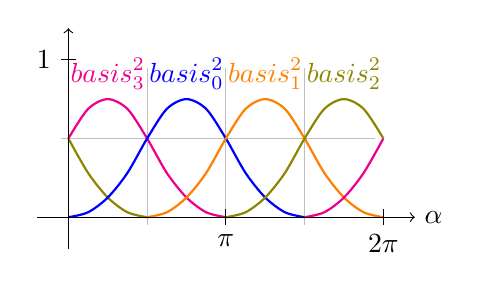
\begin{tikzpicture}
  \draw[color=lightgray] (-0.1, -0.1) grid (3.9, 1.9);

  \draw[color=blue] (1.5,1.5) node[above] {$\gls{basis}_0^2$};
  \draw[color=orange] (2.5,1.5) node[above] {$\gls{basis}_1^2$};
  \draw[color=olive] (3.5,1.5) node[above] {$\gls{basis}_2^2$};
  \draw[color=magenta] (0.5,1.5) node[above] {$\gls{basis}_3^2$};
  \draw[thick,color=magenta] plot [smooth] coordinates {(0,1)(0.25,1.375)(0.5,1.5)(0.75,1.375)(1,1)(1.25,0.5625)(1.5,0.25)(1.75,0.0625)(2,0)};
  \draw[thick,color=olive] plot [smooth] coordinates {(0,1)(0.25,0.5625)(0.5,0.25)(0.75,0.0625)(1,0)};
  \draw[thick,color=blue] plot [smooth] coordinates {(0,0)(0.25,0.0625)(0.5,0.25)(0.75,0.5625)(1,1)(1.25,1.375)(1.5,1.5)(1.75,1.375)(2,1)(2.25,0.5625)(2.5,0.25)(2.75,0.0625)(3,0)};
  \draw[thick,color=orange] plot [smooth] coordinates {(1,0)(1.25,0.0625)(1.5,0.25)(1.75,0.5625)(2,1)(2.25,1.375)(2.5,1.5)(2.75,1.375)(3,1)(3.25,0.5625)(3.5,0.25)(3.75,0.0625)(4,0)};
  \draw[thick,color=olive] plot [smooth] coordinates {(2,0)(2.25,0.0625)(2.5,0.25)(2.75,0.5625)(3,1)(3.25,1.375)(3.5,1.5)(3.75,1.375)(4,1)};
  \draw[thick,color=magenta] plot [smooth] coordinates {(3,0)(3.25,0.0625)(3.5,0.25)(3.75,0.5625)(4,1)};

  \draw[->] (-0.4, 0) -- (4.4, 0) node[right] {$\alpha$};
  \draw[->] (0, -0.4) -- (0, 2.4);
  \draw (0.1, 2) -- (-0.1, 2) node[left] {$1$};
  \draw (2, 0.1) -- (2, -0.1) node[below] {$\pi$};
  \draw (4, 0.1) -- (4, -0.1) node[below] {$2\pi$};

  \end{tikzpicture}
}
\caption[Geschlossene B-Spline-Basisfunktionen]{Illustration geschlossener Basisfunktionen $\gls{basis}_p^K \colon \left(0, 2\pi\right] \to \left[0, 1\right]$ für $P=4$ gleichmäßig verteilter Kontrollpunkte, einmal mit lokaler Kontrollierbarkeit $K=1$ (a) und einmal mit $K=2$ (b).}
\label{fig:bspline}
\end{figure}


Die Definitionen~\eqref{eq:bspline_basis_init} und~\eqref{eq:bspline_basis_schritt} der Basisfunktionen sind lediglich für offene B-Spline-Kurven konzipiert.
Im Kontext von Winkeln müssen wir die Basisfunktionen $\gls{basis}_p^K\left(\alpha\right)$ aber insofern modifizieren, dass diese eine geschlossene Kurve beschreiben können.
Abbildung~\ref{fig:bspline} soll dabei das Konzept geschlossener Basisfunktionen auf Winkeln veranschaulichen.
Mit der expliziten Forderung gleichmäßig verteiler Knoten im Intervallbereich ergibt sich dann der Knotenvektor $\ve{\tau} \coloneqq {\left[\alpha_0, \ldots, \alpha_{P+K}\right]}^{\top} \in \gls{R+}^{P+K+1}$ mit $\alpha_p \coloneqq 2\pi p/P$.
Damit kann $\gls{basis}_p^K\left(\alpha\right)$ modifiziert werden zu
\begin{equation}
\begin{split}
  \gls{basis}_p^0\left(\alpha\right) \coloneqq & \begin{cases}
    1, \text{wenn } \alpha \in \left(\alpha_p, \alpha_{p+1}\right],\\
    0, \text{sonst}
  \end{cases}\\
  \gls{basis}_p^k\left(\alpha\right) \coloneqq & \frac{\alpha - \alpha_p}{\alpha_{p+k} - \alpha_p} \gls{basis}_p^{k-1}\left(\alpha\right) + \frac{\gls{modulo}\left(\alpha_{p+k+1}, 2\pi\right) - \alpha}{\alpha_{p+k+1} - \alpha_{p+1}}\gls{basis}_{\gls{modulo}\left(p+1,P\right)}^{k-1}\left(\alpha\right),
\end{split}
\label{eq:bspline_basis_winkel}
\end{equation}
indem die Indexierungen des Knotenvektors und der Basisfunktion im rechten Summanden im Vergleich zu~\eqref{eq:bspline_basis_schritt} über den Modulo-Operator $\gls{modulo}\left(a,b\right) \coloneqq a - qb$ mit $\gls{modulo}\left(a,b\right) < b$ für $a,b\in \gls{R+}$, $q \in \gls{N}$ angepasst werden.
$\gls{basis}_p^K$ setzt sich dabei analog aus den Basisfunktionen$\gls{basis}_p^K$ und $\gls{basis}_{p+1}^K$ zusammen, \dhe{} den Basisfunktionen der betrachteten Partition und der rechts darauf folgenden.
Für die aktuelle Partition $p$ im linken Summanden muss keine Veränderung vorgenommen werden und kann analog zu~\eqref{eq:bspline_basis_schritt} übernommen werden.
Lediglich im rechten Summanden muss darauf geachtet werden, \enquote{nicht über die Grenzen hinaus zu laufen}.
Für den Grenzfall $p = P-1$ wird daher im zweiten Summanden die Basisfunktion $\gls{basis}_0^{k-1}\left(\alpha\right)$ addressiert.
Analog muss der Zähler des Koeffizienten auf den korrekten Winkel von $\alpha_{p+k+1}$ verweisen.
Für die Nenner muss aufgrund der streng monotonen Definition des Knotenvektors $\ve{\tau}$ keine Änderung vorgenommen werden.

\paragraph{Faltungsoperator}
\label{bspline_faltungsoperator}

Es kann folglich analog zu~\eqref{eq:partitionierung_faltung} der Faltungsoperator $\ve{f}_{\mathrm{in}} \star \ve{\hat g}$ auf Basis eines stückweisen polynomiellen Filters beschrieben werden.
Mit $\gls{Adisttilde} \in \gls{R}^{N \times N}$ und $\gls{Ddisttilde} \in \gls{R}^{N \times N}$ ergibt sich $\ve{f}_{\mathrm{in}} \star \ve{\hat g}$ dann als
\begin{equation*}
  \ve{f}_{\mathrm{in}} \star \ve{\hat g} \approx c_P \gls{Ddisttilde}^{-1}\ve{f}_{\mathrm{in}} + \sum_{p=0}^{P-1} \left(\left(c_p \gls{basis}_p^K\left(\gls{Arad}\right)\right)\gls{hadamard}\left(\gls{Ddisttilde}^{-\frac{1}{2}}\gls{Adisttilde}\gls{Ddisttilde}^{-\frac{1}{2}}\right)\right)\ve{f}_{\mathrm{in}}
\end{equation*}
mit den freien Parametern ${\left[c_0, \ldots, c_P\right]}^{\top} \in \gls{R}^{P+1}$, wobei $\gls{basis}_p^K$ elementweise auf die Matrix \gls{Arad} angewendet wird.
$\ve{f}_{\mathrm{in}} \star \ve{\hat g}$ sammelt dabei die aktuellen Merkmale an den einzelnen Knoten über $c_P \gls{Ddisttilde}^{-1}\ve{f}_{\mathrm{in}}$ und aggreriert diese mit den Merkmalen der lokalen Nachbarschaft über den polynomiellen Filter $\left(c_p\gls{basis}_p^K \left(\gls{Arad}\right)\right) \gls{hadamard} \left(\gls{Ddisttilde}^{-1/2}\gls{Adisttilde}\gls{Ddisttilde}^{-1/2}\right)$, der so die Länge und Richtungen der Kanten berücksichtigt.
Für $K=0$ ist die Faltung über den B-Splines äquivalent zu der Faltung über den Partitionen des Graphen aus~\eqref{eq:partitionierung_faltung} aufgrund der Rechteckfunktionen ${\left\{\gls{basis}_p^0\left(\alpha\right)\right\}}_{p=0}^{P-1}$.

\paragraph{Implementierung}
\label{bspline_implementierung}

Für Merkmalsmatrizen $\ma{F}_{\mathrm{in}} \in \gls{R}^{N \times M_{\mathrm{in}}}$ und $\ma{F}_{\mathrm{out}} \in \gls{R}^{N \times M_{\mathrm{out}}}$ kann die Faltung über einem Filtertensor $\gls{W} \in \gls{R}^{\left(P+1\right) \times M_{\mathrm{in}} \times M_{\mathrm{out}}}$ als
\begin{equation*}
  \ma{F}_{\mathrm{out}} \coloneqq \gls{Ddisttilde}^{-1}\ma{F}_{\mathrm{in}}\gls{W}_{P+1} + \sum_{p=0}^{P-1} \left(\gls{basis}_p^K\left(\gls{Arad}\right) \gls{hadamard}\left(\gls{Ddisttilde}^{-\frac{1}{2}}\gls{Adisttilde}\gls{Ddisttilde}^{-\frac{1}{2}}\right)\right)\ma{F}_{\mathrm{in}}\ma{W}_{p+1}
\end{equation*}
beschrieben werden.
Im Vergleich zu Kapitel~\eqref{partitionierung_implementierung} erhöht sich der Aufwand der Faltung zu $\gls{O}\left(KPM_{\mathrm{in}}M_{\mathrm{out}}\right)$, da die Partitionen der Adjazenzmatrizen nicht mehr disjunkt, sondern $\left(K+1\right)$-mal betrachtet werden.

\begin{figure}[t]
\centering
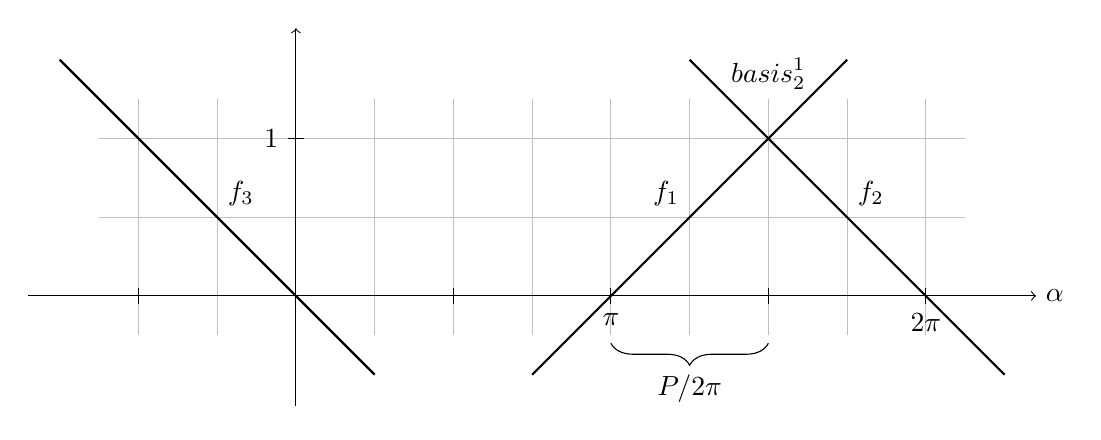
\begin{tikzpicture}
  \draw[color=lightgray] (-2.5, -0.5) grid (8.5, 2.5);

  \draw[thick] (3, -1) -- node[shift={(-0.3,0.3)}] {$f_1$} (7, 3);
  \draw[thick] (9, -1) -- node[shift={(0.3,0.3)}]  {$f_2$} (5, 3);
  \draw[thick] (1, -1) -- node[shift={(0.3,0.3)}]  {$f_3$} (-3, 3);

  \draw[->] (-3.4, 0) -- (9.4, 0) node[right] {$\alpha$};
  \draw[->] (0, -1.4) -- (0, 3.4);
  \draw (0.1, 2) -- (-0.1, 2) node[left] {$1$};
  \draw (-2, 0.1) -- (-2, -0.1);
  \draw (2, 0.1) -- (2, -0.1);
  \draw (4, 0.1) -- (4, -0.1) node[below] {$\pi$};
  \draw (6, 0.1) -- (6, -0.1);
  \draw (8, 0.1) -- (8, -0.1) node[below] {$2\pi$};

  \draw (6,2.5) node[above] {$\gls{basis}_2^1$};

  \draw [decoration={brace,mirror,amplitude=8pt},decorate] (4,-0.6) -- node[below=8pt] {$P/2\pi$} (6,-0.6);
\end{tikzpicture}
\caption[B-Spline-Funktion mit $K=1$ über Minimum-Maximumfunktion]{Beweisidee zur \enquote{kreisförmigen} Dreiecksfunktion für B-Spline-Funktionen mit $K=1$ und $P=4$ als Darstellung über eine Minimum-Maximumfunktion auf drei Geraden, hier illustriert am Beispiel $\gls{basis}_2^1$.}
\label{fig:bspline_beweis}
\end{figure}


Für $K=1$ lässt sich weiterhin die \enquote{kreisförmige} Dreiecksfunktion $\gls{basis}_p^1\left(\alpha\right)$ aus einer Reihe von Minimum- und Maximumfunktionen effizient implementieren.
So gilt, dass $\gls{basis}_p^1\left(\alpha\right)$ zu
\begin{equation*}
  \begin{split}
    \gls{basis}_p^1\left(\alpha\right) = \max \Big( & \min \left( \max\left(\frac{P}{2\pi}\alpha - p, 0\right), \max\left(-\frac{P}{2\pi}\alpha + p + 2, 0\right)\right),\\
    & \max\left(-\frac{P}{2\pi}\alpha + p + 2 - P, 0\right) \Big)
  \end{split}
\end{equation*}
vereinfacht werden kann.
Dies lässt sich verifizieren, in dem die kreisförmige Dreiecksfunktion im Intervall $\left(0, 2\pi\right]$ als Verknüpfung dreier Geraden verstanden wird — zwei Geraden, die das Dreieck im Intervall $\left(2\pi p/P, 2\pi \left(p+2\right)/P\right]$ aufspannen, und einer absteigenden Geraden, die um $2\pi$ nach links verschoben wurde und dafür sorgt, die Basisfunktion für $p=P-1$ kreisförmig abzuschließen und in allen anderen Fällen keinen Anteil im Gültigkeitsbereich der Funktion $\gls{basis}_p^1 \colon \left(0,2\pi\right] \to \left[0,1\right]$ besitzt (\vgl{} Abbildung~\ref{fig:bspline_beweis}).
Den Geraden kann die Steigung $P/2\pi$ \bzw{} $-P/2\pi$ zugeordnet werden und sie können damit folglich über
\begin{equation*}
\begin{split}
  f_1\left(\alpha\right) \coloneqq & \frac{P}{2\pi}\left(\alpha - 2\pi\frac{p}{P}\right) = \frac{P}{2\pi}\alpha - p\\
  f_2\left(\alpha\right) \coloneqq & - \frac{P}{2\pi}\left(\alpha - 2\pi\frac{p+2}{P}\right) = - \frac{P}{2\pi}\alpha + p + 2\\
  f_3\left(\alpha\right) \coloneqq & - \frac{P}{2\pi}\left(\alpha - 2\pi\frac{p+2}{P} + 2\pi\right) = - \frac{P}{2\pi}\alpha + p + 2 - P
\end{split}
\end{equation*}
beschrieben werden.
Mittels $\max\left(f_i\left(\alpha\right), 0\right) \in \gls{R+}$ können diese auf den positiven reellen Raum eingegrenzt werden.
$f_{\triangle} \coloneqq \min\left(\max\left(f_1, 0\right), \max\left(f_2, 0\right)\right)$ beschreibt damit die Dreiecksfunktion, indem sie sich stets für das Minimum von $\max\left(f_1, 0\right)$ \bzw{} $\max\left(f_2,0\right)$ entscheidet.
Folglich beschreibt $\max\left(\max\left(f_3,0\right), f_{\triangle}\right)$ die Basisfunktion $\gls{basis}_p^1$ im Intervall $\left(0, 2\pi\right]$ für alle $p \in \left\{0, \ldots, P-1\right\}$.
